% gr-MysticRose.tex -- the complete graph K24 ; the colour of an edge
% gives the distance between its ends along the circle.
% Engine : pdfLaTeX or LuaLaTeX
\documentclass[border=3mm, convert=false]{standalone}
\usepackage{xcolor}
\usepackage{tkz-berge}
\begin{document}
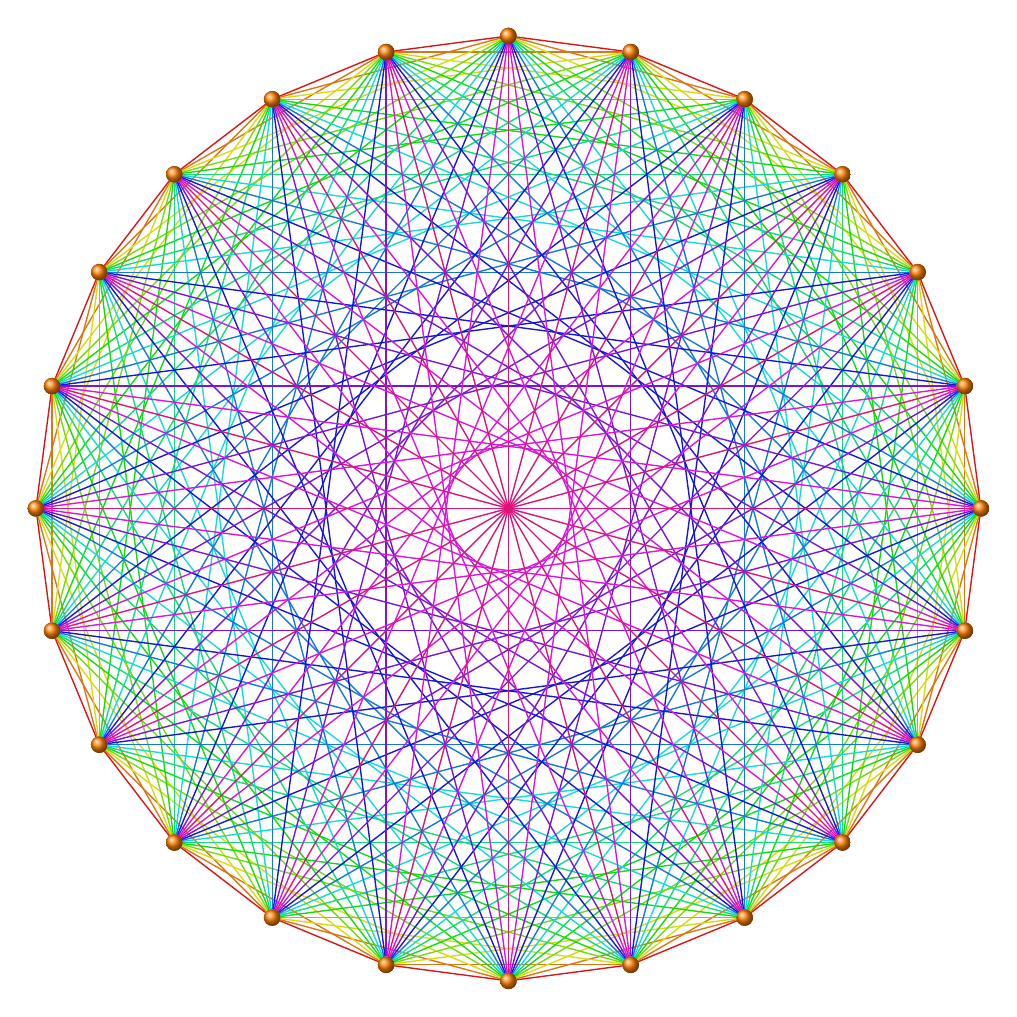
\begin{tikzpicture}
  \GraphInit[vstyle=Art]
  \SetVertexNoLabel
  \tikzset{VertexStyle/.append style = {minimum size = 6pt}}
  \grEmptyCycle[RA=6]{24}
  \foreach \d in {1,...,12}{%
    \pgfmathsetmacro\hue{(\d-1)/12}
    \definecolor{h}{hsb}{\hue,0.9,0.85}
    \colorlet{c}[rgb]{h}
    \pgfmathtruncatemacro\m{\d==12 ? 11 : 23}
    \foreach \i in {0,...,\m}{%
      \pgfmathtruncatemacro\j{mod(\i+\d,24)}
      \Edge[local,color=c,lw=.5pt](a\i)(a\j)}}
  \grEmptyCycle[RA=6]{24}
\end{tikzpicture}
\end{document}
